\begin{frame}{Embedded Systeme}
	\footnotesize{
	\begin{multicols}{2}
				\only<handout>{Digitales Multimeter}
				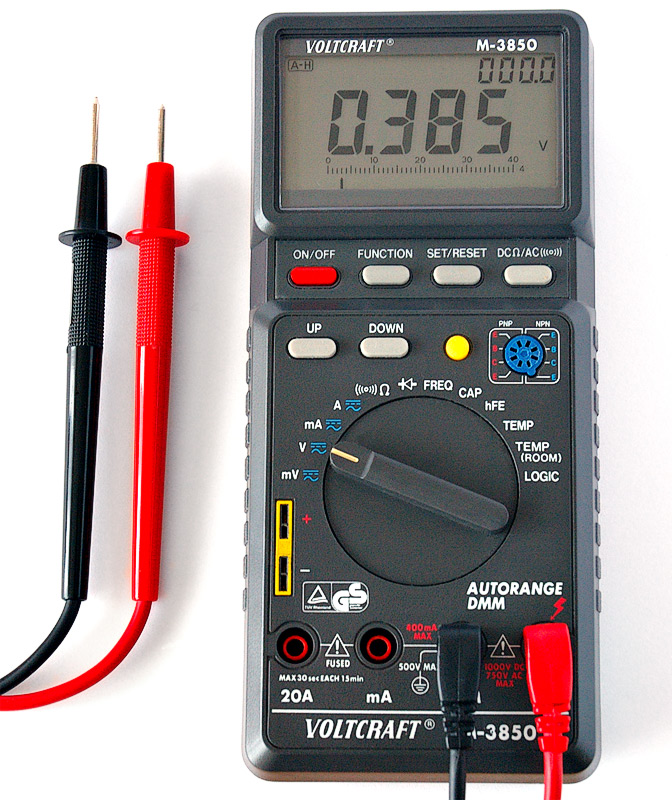
\includegraphics[height=4cm]{res/Digital_Multimeter_Aka.jpg}\hcite{multimeter}
				\only<handout>{
					\begin{itemize}
						\item Sensor produziert ~20 B/sec
						\item Reduzierung auf ~2 B/sec
						\item Verarbeitung auf internem uC
					\end{itemize}
				}
				\pagebreak
				\only<handout>{ATLAS/LHC/CERN}
				\visible<2->{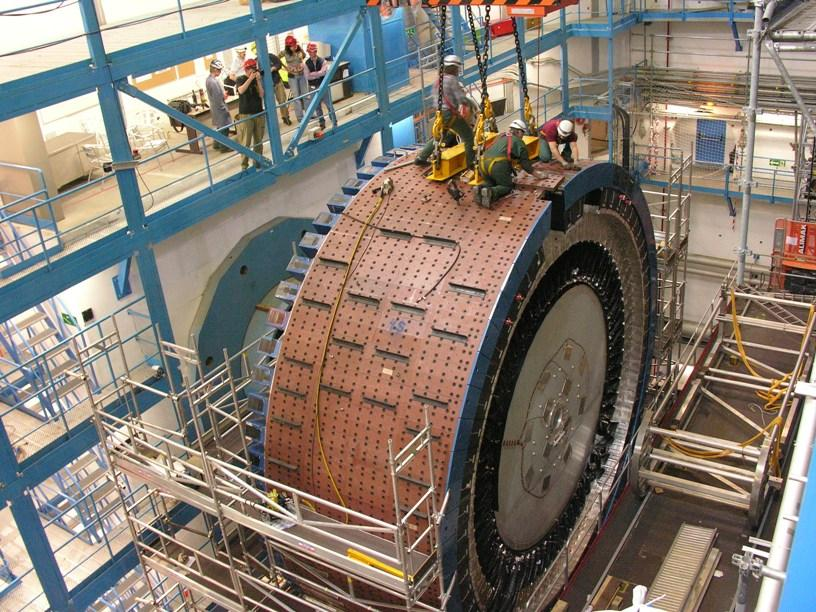
\includegraphics[height=4cm]{res/ATLAS_Tile_Calorimeter}\hcite{tileCalorimeter}}
				\only<handout>{
					\begin{itemize}
						\item Sensor produziert 1 PiB/sec
						\item Reduzierung auf ~100 MiB/sec \hcite{wikiAtlas}
						\item Verarbeitung auf eigenen 20'000 Server und Grid \hcite{wikiCernServer}
					\end{itemize}
				}
	\end{multicols}
	}
\end{frame}

\begin{frame}{Firmware}
	``Unter Firmware versteht man Software, die in elektronische Geräte eingebettet ist.'' \cite{wikiFirmware}
	
	\begin{itemize}
		\item Gesamtes Software-Image von Embedded System
		\item Software für Subsysteme
		\begin{itemize}
			\item Power Management
			\item WLAN Karte
			\item BIOS
			\item Touch-Screen
		\end{itemize}
	\end{itemize}
\end{frame}

\begin{frame}{PID 1}
	Nachdem Linux alles initialisiert hat wird Kontrolle an Userspace übergeben.
	Üblicherweise ist dies systemd.
	\begin{itemize}
		\item systemd
		\begin{itemize}
			\item einfach da bekannt
			\item wenn mehrere Dienste nötig
			\item gewisse Grösse
		\end{itemize}
		\item Script
		\begin{itemize}
			\item wenn nur wenige Dienste
		\end{itemize}
		\item Applikation
		\begin{itemize}
			\item Applikation muss alles machen
			\item nur für monolithische Applikationen
		\end{itemize}
	\end{itemize}
\end{frame}

\begin{frame}{Yocto}
	Aufgaben um Embedded system zu erstellen
	\begin{itemize}
		\item Cross Compiler bauen
		\item sysfs bauen (Kernel und benötigte Tools für System)
		\item Cross Compiler und sysfs für Developer bereitstellen (SDK)
	\end{itemize}
	Aufgaben um Embedded system zu deployen
	\begin{itemize}
		\item Applikation cross-compilen
		\item sysfs cross-compilen
		\item Kernel cross-compilen
		\item Applikationen paketieren
		\item Image zusammenstellen
	\end{itemize}
\end{frame}

\begin{frame}{Kernel / Linux}
	\begin{itemize}
		\item Verteilen von Ressourcen
		\item Initialisieren und Abstrahieren der Hardware
	\end{itemize}
\end{frame}

